\chapter{Lösungsansatz zur Klassifikation}
In diesem Kapitel geht es um die Strategie, wie eine Klassifikation der
Hunderassen für den großen (120 Klassen) und den kleinen (5 Klassen) Datensatz
mittels mehrerer Neuronaler Netze und eines Random Forest erreicht werden kann.

\section{Größe der Bilder}
\label{sec:größe-bilder}
Höhe und Breite der Bilder sind unterschiedlich im großen Datensatz, wie in
\autoref{fig:scatter_groß} dargestellt.

\begin{figure}
  \centering
  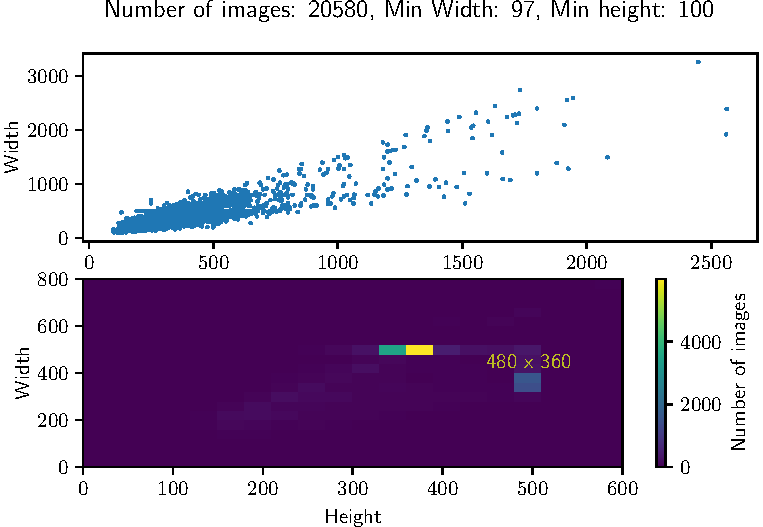
\includegraphics[scale=0.9]{pics/width_height_scatter_hist2d.pdf}
  \caption{Oben: Scatter-Plot der Höhen- und Breitenverteilung der Bilder aus dem großen Datensatz.
  Unten: Zweidimensionales Histogramm der Höhen- und Breitenverteilung.
  Die gelbe Größe entspricht der am häufigsten auftretenden Kombination
  aus Breite und Höhe.}
  \label{fig:scatter_groß}
\end{figure}

Die minimale Breite liegt bei 97 Pixeln und die minimale Höhe bei 100 Pixeln
bzw. für den kleinen Datensatz bei 125x138 Pixeln. Prinzipiell arbeiten die
verwendeten Neuronalen Netze ohne definierte Input size, allerdings müssen die
Bilder auf eine Größe gebracht werden, da \texttt{numpy arrays} eine definierte
Größe haben müssen und im Verlaufe des Trainings \texttt{numpy arrays} verwendet
werden. Eine Möglichkeit wäre es nun, alle Bilder auf diese minimale Größe zu
resizen. Damit würde allerdings ein Informationsverlust einhergehen. Aus diesem
Grund wurde für \MiniDog (mehr dazu in \autoref{sec:netzwerk}) ein zu Teilen
selbstgeschriebener \texttt{Datagenerator} verwendet, der die Bilder batchwise
lädt und batchwise auf das Minimum im Batch resized. Auf diese Weise ist der
Informationsverlust geringer als alle Bilder auf 125x138 zu resizen.

In \autoref{fig:scatter_klein} ist die Höhen- und Breitenverteilung auch für
den kleinen Datensatz dargestellt.

\begin{figure}
  \centering
  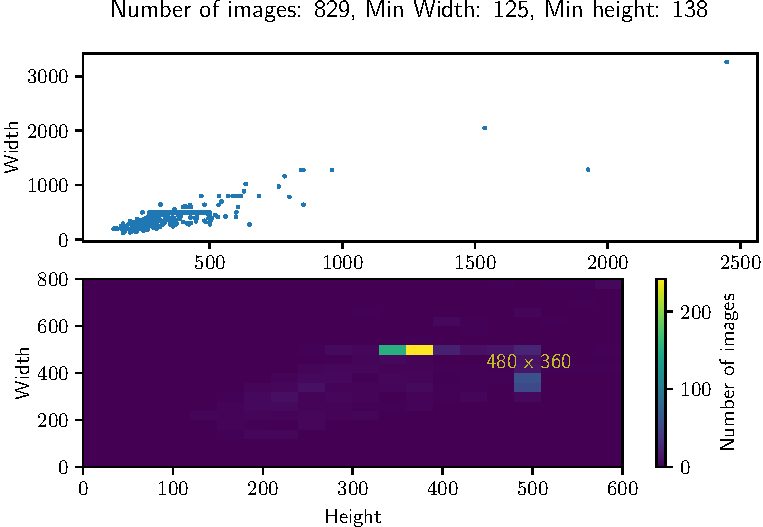
\includegraphics[scale=0.9]{pics/width_height_scatter_hist2d_klein.pdf}
  \caption{Oben: Scatter-Plot der Höhen- und Breitenverteilung der Bilder aus
  dem kleinen Datensatz.
  Unten: Zweidimensionales Histogramm der Höhen- und Breitenverteilung.
  Die gelbe Größe entspricht der am häufigsten auftretenden Kombination
  aus Breite und Höhe.}
  \label{fig:scatter_klein}
\end{figure}

Für \PreDog und \PreBig (mehr in \autoref{sec:netzwerk}) muss aufgrund der
vortrainierten Netze eine feste Größe der Bilder gewählt werden. Wegen
technischen Schwierigkeiten konnte nicht auf die minimale Größe des großen
Datensatzes trainiert  werden. Stattdessen wurde auf die minimale Größe des
kleinen Datensatzes resized. Da nur maximal 71 Bilder des großen Datensatzes
eine kleinere Größe haben als 125x138, fällt dies nicht allzu sehr ins Gewicht.

\section{Data Augmentation}
Wie bereits in \autoref{chap:datensatz} dargestellt, entfallen auf jede Klasse
nur ungefähr 150 Bilder, was eine sehr geringe Statistik darstellt. Aus diesem
Grund wurde Data Augmentation verwendet. Das bedeutet, dass bei jedem neuen
Aufruf des \texttt{Datagenerators} nach dem Resizen das Bild um einen zufälligen
Winkel zwischen \SI{-30}{\degree} und \SI{30}{\degree} rotiert wird. Dabei
aufstehende Leerflächen werden geschwärzt. Dann wird mit \SI{50}{\percent}
Wahrscheinlichkeit das Bild in x- und y-Richtung verschoben oder ein Zoom in x-
und y-Richtung durchgeführt. Damit bei diesen Transformationen der Hund noch
immer komplett zu sehen ist und nicht z.\,B. durch die Verschiebung nur noch ein
Teil des Hundes zu sehen ist, wird vorher aufgrund der Bounding Boxes, die im
Datensatz gegeben sind, das Zoom- bzw. Translationslimit bestimmt.

Drei Beispiele sind in \autoref{fig:data_augmentation} zu sehen.

\begin{figure}
  \centering
  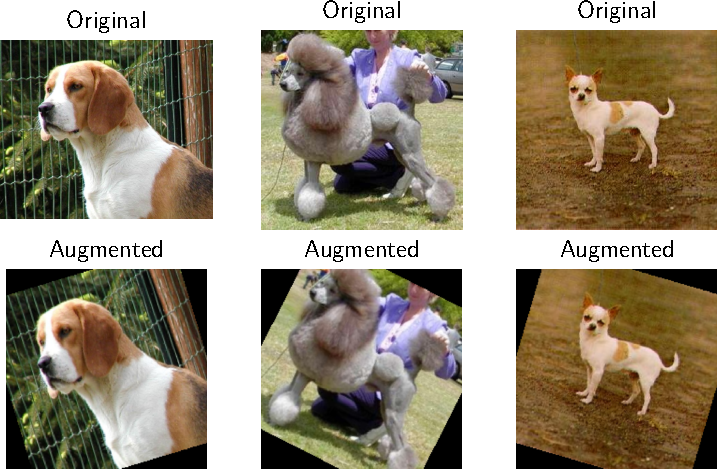
\includegraphics[width=\the\textwidth]{pics/subplot.pdf}
  \caption{Beispielbilder zur Data Augmentation. In der oberen Zeile sind die
  Originalbilder aus dem Datensatz und unten die Bilder nach dem Resizen und der Data Augmentation.}
  \label{fig:data_augmentation}
\end{figure}

Da der Datagenerator nach jeder Epoche neu aufgerufen wird, sehen die
Trainingsbilder in jeder Epoche anders aus, was allgemein die Robustheit des
\CNN gegenüber Translation, Rotation, etc. der Bilder erhöht und nebenbei mehr
Statistik generiert, da die Bilder immer anders aussehen.

\section{Netzwerkstrukturen}
\label{sec:netzwerk}
Insgesamt wurden drei verschiedene Netzwerkarchitekturen verwendet, namentlich
\MiniDog, \PreDog und \PreBig. Die letzten beiden Architekturen verwenden dabei
ein vortrainiertes Netz mit Namen \texttt{InceptionResNetV2}. Dieses ist bei
Keras vorimplementiert \cite{inception} und wurde auf \texttt{ImageNet}
trainiert, einem Datensatz insgesamt bestehend aus 14197122 Bildern
\cite{imagenet}.

Da \texttt{InceptionResNetV2} alleine bereits 55873736 freie Parameter hat, muss
bei \PreBig und \PreDog Regularisierung verwendet werden. Die Struktur ist für
beide Neuronalen Netze die gleiche: An \texttt{InceptionResNetV2} ist eine Lage
\texttt{AveragePooling2D} mit einer \texttt{Poolsize=(4, 4)} und eine Lage
\texttt{GlobalMaxPooling2D} angeschlossen, um die Anzahl der freien Parametern
zu reduzieren. Danach kommen drei \texttt{Dense}-Layer, mit den
Dimensionalitäten 30, 30, 5 (für \PreDog) und 150, 120, 120 für \PreBig. Die
Layern sind \texttt{L2-Regularisiert} mit einem Wert von 0.01 für \PreDog und
0.007 für \PreBig. Außerdem befinden sich je ein \texttt{Dropout}-Layer mit
einer Stärke von 0.2 (\PreDog) bzw. 0.15 (\PreBig) zwischen den
\texttt{Dense}-Layern. Die Aktivierungsfunktion der \texttt{Dense}-Layer ist
\texttt{PReLU}, die Initialisierung wurde nach der von Kaiming He entwickelten
Methode durchgeführt \cite{tensowflow-he}, so wie in \cite{he-ini} empfohlen.
Auch die Gewichte des Kernels der \texttt{Dense}-Layer wurden nach der von
Kaiming He entwickelten Methode initialisiert. \texttt{PReLU} ist eine
modifizierte Version von \texttt{ReLU}, die sich dadurch auszeichnet, dass die
Funktion $f(y)$ für negative $y$ nicht 0 ist wie bei \texttt{ReLU}, sondern $ay$
mit einem Koeffizienten $a$, der adaptiv angepasst wird \cite{prelu}. Die
Aktivierungsfunktion des letzten \texttt{Dense}-Layers ist \texttt{softmax}.

Außerdem wurde ein Neuronales Netz ohne vortrainiertes Netz verwendet, dies heißt
\MiniDog. Die Struktur ist in \autoref{fig:struktur_minidognn} abgebildet.

\begin{figure}
  \centering
  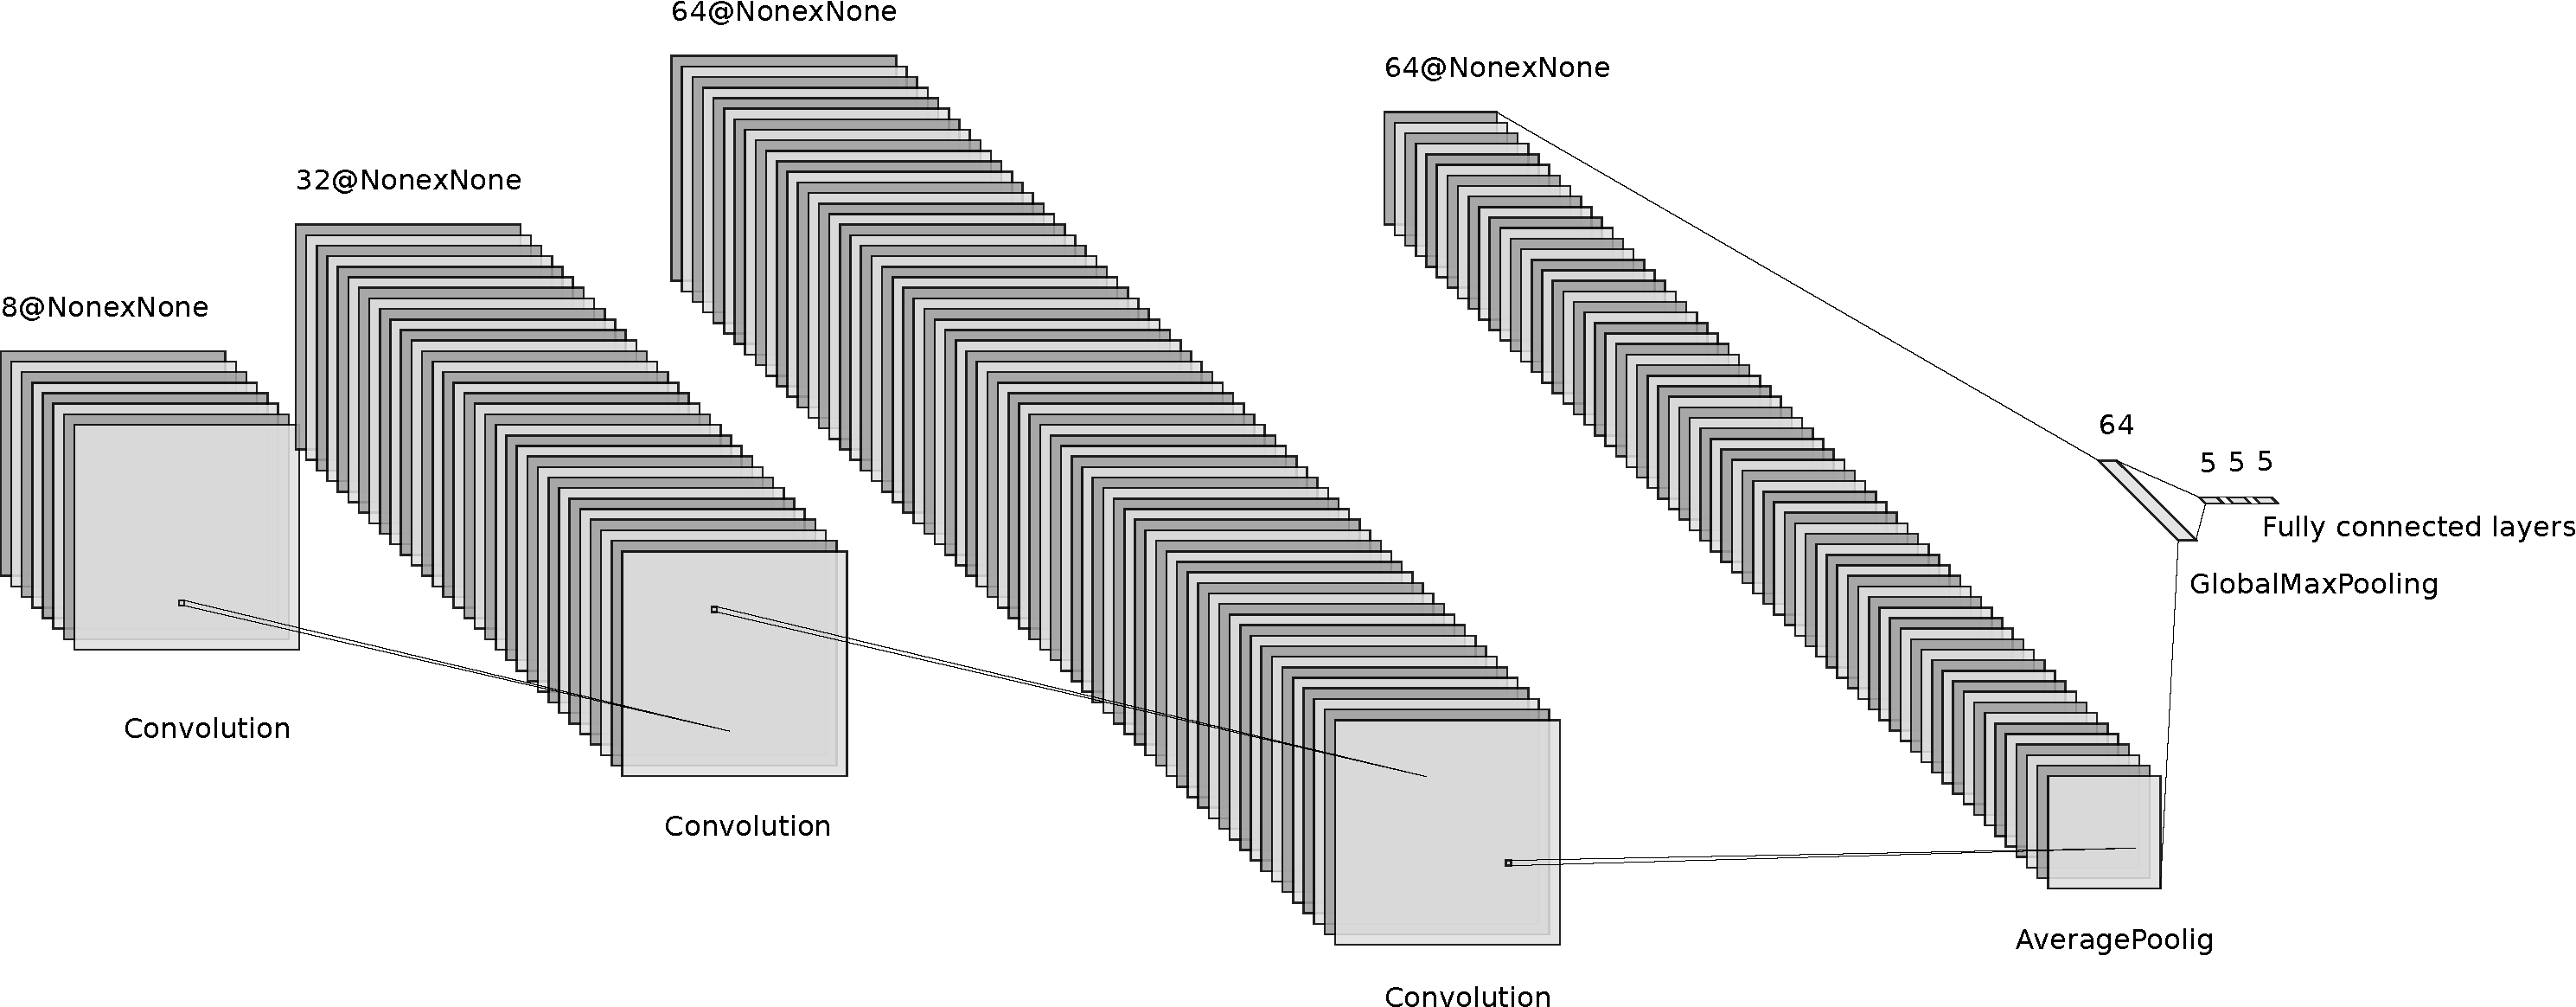
\includegraphics[width=\textwidth]{pics/nn.pdf}
  \caption{Struktur des Neuronalen Netzes \MiniDog. Die Dimensionalität
  der \texttt{Dense}-Layer richtet sich nach der Anzahl der Klassen im verwendeten Datensatz.}
  \label{fig:struktur_minidognn}
\end{figure}

Wie schon bei \PreDog und \PreBig wird für die \texttt{Dense}-Layer und auch
für die \texttt{Convolutional}-Layer wird die von Kaiming He entwickelte Methode
zur Initialisierung der Gewichte verwendet. Ebenso wird \texttt{PReLU} als
Aktivierungsfunktion genutzt für beide Arten von Layern. Außerdem wird
\texttt{L2-Regularisierung} für alle Arten von Layern genutzt.

Als letzte Netzwerkstruktur wird der Autoencoder und der dazugehörige Random
Forest vorgestellt. Der Encoder des Autoencoders besteht aus vier
\texttt{Convolutional}-Layern mit drei \texttt{MaxPooling}-Layern dazwischen,
die die Anzahl der Parameter reduzieren, sodass die Bilder am Ende des Encoders
statt als dreidimensionales Array als Vektor vorliegen. Der Decoder besteht aus
fünf \texttt{Convolutional}-Layern und drei \texttt{UpSampling2D}-Layern, die
zwischen den ersten vier \texttt{Convolutional}-Layern platziert sind. Auf diese
Weise wird aus dem Vektor mit den Features wieder ein dreidimensionales Array.
Die Aktivierungsfunktionen der \texttt{Convolutional}-Layer ist \texttt{ReLU},
bis auf den letzten, dort wird \texttt{Sigmoid} verwendet. Zu den
Hyperparametern lässt sich nicht viel sagen an dieser Stelle, da ein
\texttt{Grid Search} verwendet wurde, um diese zu optimieren, siehe
\autoref{sec:hyperparam}.

\section{Hyperparameter-Optimierung}
\label{sec:hyperparam}
Für \MiniDog und der Random Forest wurde eine Hyperparameter-Optimierung in Form
eines \texttt{Grid Search} durchgeführt. Allerdings wurde im Falle von \MiniDog
eine selbgeschriebene Funktion verwendet, die aus Zeitgründen auf die
\texttt{Cross Validation} verzichtet. Auch werden nur drei Hyperparameter
optimiert: Die Stärke der \texttt{L2-Re\-gu\-la\-ri\-sier\-ung}, die
\texttt{Batch-Size} und das Verwenden der Farbinformationen. Beim letzten Punkt
werden die Bilder einmal in schwarz-weiß und einmal mit Farbinformationen
eingelesen, um zu prüfen, wie wichtig dieser Parameter für das Neuronale Netz
ist.

Für den RF wurden \texttt{GridSearchCV} mit einer dreifachen Kreuzvalidierung genutzt.
Unter anderem wurde die maximale Tiefe oder die Anzahl an Schätzern optimiert.

% \begin{table}
%   \caption{Optimierte Hyperparameter für den RF}
%   \label{tab:hyper_rf}
%   \begin{tabular}{c c c c c c}
%     \toprule
%     max\_features & max\_depth & min\_samples\_leaf & min\_samples\_split & criterion & n\_estimators \\
%     \midrule
%     auto, log2 & None, 10, 100 & 1, 10 31 & 2, 8, 10 & gini, entropy & 100, 400, 1000, 1500 \\
%     \bottomrule
%   \end{tabular}
% \end{table}

Für eine Hyperparameteroptimierung von \PreBig und \PreDog war die Hardware nicht stark genug.
